\chapter{Ejemplos}
En este capítulo veremos algunos ejemplos de iteraciones de funciones racionales
para introducirnos en la rama de la Dinámica Compleja.

% --- SECCIÓN ------------------------------------------------------------------
% --- TRANSFORMACIONES DE MÖBIUS -----------------------------------------------
\section{Transformaciones de Möbius}
Comencemos con el caso más sencillo, las funciones racionales de grado $1$.
Estas funciones se conocen como transformaciones de Möbius y su dinámica puede
describirse de forma bastante explícita.

\begin{definicion}[Transformación de Möbius]
    Una transformación de Möbius es una función racional de la forma
    \[
        R(z) = \frac{az+b}{cz+d}, \quad ad-bc \ne 0
    \] 
    donde $z$, $a$, $b$, $c$, $d$ son números complejos. Además, seguiremos los
    siguientes convenios con el punto del infinito: $R(\infty)=a/c$ y $R(-c/d) =
    \infty$.
\end{definicion}

Veamos primero la transformación de Möbius
\begin{equation}\label{eq:mobiusEj1}
    R(z) = \frac{3z-2}{2z-1}.
\end{equation}

Esta función tiene un único punto fijo, $\zeta = 1$, y este es indiferente
porque $R'(1) = 1$. La pregunta que nos hacemos es: si iteramos en un punto
arbitrario del plano complejo, $z$, ¿cómo se comportará la secuencia $R^n(z)$?

\begin{definicion}[Órbita]
    Dados una función, $R \colon \ExtC \to \ExtC$, y un punto inicial, $z_0 \in
    \ExtC$, llamamos órbita de $z_0$ a la sucesión $(z_n)_{n \in \mathbb{N}}$
    donde $z_n = R^n(z_0)$.
\end{definicion}

En este caso, y en general para todas las transformaciones de Möbius, se pueden
encontrar expresiones explícitas de $R^n(z)$ de forma sistemática. Esto facilita
mucho el análisis del comportamiento de sus órbitas.

Volviendo a la transformación de Möbius con la que estamos trabajando
(\ref{eq:mobiusEj1}), se puede comprobar que
\[
    R^n(z) = \frac{(2n+1)z-2n}{2nz-(2n-1)} =  1 + \frac{z-1}{2nz-(2n-1)}.
\]
Así, es claro que para todo $z \neq \zeta$, $R^n(z) \to \zeta$: el denominador
crece linealmente con $n$, mientras que el numerador permanece constante.
También, $R^n(\zeta) \to \zeta$ porque $R(\zeta) = \zeta$. Por tanto, tenemos
que en general
\[
    R^n(z) \to \zeta,
\]
cuando $n \to \infty$. Es decir, en este ejemplo todas las órbitas convergen al
único punto fijo $\zeta$.

Consideremos ahora una transformación con un comportamiento distinto:
\[
    R(z) = \frac{(1+i)z + (1-i)}{(1-i)z + (1+i)},
\]
que tiene dos puntos fijos, $\zeta_1 = 1$ y $\zeta_2 = -1$, ambos indiferentes.

Para simplificar el estudio del comportamiento de las órbitas de esta
transformación vamos a estudiar el de las órbitas de una función conjugada. Para
nuestra transformación, se puede comprobar que
\[
    R(z) = g^{-1}Sg(z),
\]
con
\begin{align*}
    S(z) &= -iz, \\
    g(z) &= \frac{1+z}{1-z};
\end{align*}
es decir, $R$ es conjugada a la rotación $S(z)=-iz$.

Como $(-i)^4=1$, se tiene $S^4(z)=z$ para todo $z$. En consecuencia,
\[
    R^4(z)=\Id(z)=z,
\]
para todo $z \in \ExtC$. Así, todas las órbitas son periódicas de período que
divide a $4$. Además, $S(z) \neq z$ excepto para los puntos fijos, luego las
órbitas de puntos no fijos no convergen.

Estos dos ejemplos ilustran bien la variedad de comportamientos que ya aparecen
en grado $1$: convergencia hacia un punto fijo en el primer caso y dinámica
periódica en el segundo. En general, los comportamientos de las órbitas de las
transformaciones de Möbius pueden clasificarse según las trasnformaciones tengan
uno o dos puntos fijos.

\begin{teorema}
Sea $R$ una transformación de Möbius, si $R$ tiene
\begin{enumerate}
    \item un punto fijo, $\zeta$, entonces para todo $z \in \ExtC$, $R^n(z) \to
        \zeta$ cuando $n$ tiende a $\infty$;
    \item dos puntos fijos, entonces para todo $z \in \ExtC$ se tiene que cuando
        $n$ tiende a $\infty$
    \begin{enumerate}
        \item $R^n(z)$ converge a uno de los puntos fijos,
        \item $R^n(z)$ se mueve cíclicamente en un conjunto finito de puntos,
        \item o $R^n(z)$ forma un subconjunto denso de un círculo o recta.
    \end{enumerate}
\end{enumerate}
\end{teorema}

\begin{proof}
    Véase \cite[4--5]{Beardon1991}.
\end{proof}

% --- SECCIÓN ------------------------------------------------------------------
% --- POLINOMIOS DE GRADO 2 ----------------------------------------------------
\section{Polinomios de grado 2}
Pasemos a analizar el comportamiento de polinomios de grado 2. Inicialmente
puede parecer que son incluso más sencillos que las transformaciones de Möbius,
pero pronto nos damos cuenta de que este no es el caso. Empecemos examinando el
polinomio de grado dos más sencillo,
\[
    R(z) = z^2.
\]

Sus puntos fijos son $0$ (atractor), $1$ (repulsor), e $\infty$ (atractor). Es
más, para todo $z$ tal que $|z| < 1$,  su órbita converge a $0$; y si $|z| > 1$,
su órbita converge a $\infty$ (ver Figura~
\ref{fig:z_squared_fatou_basins_and_times}). Pero, ¿qué ocurre en los puntos de
la circunferencia unidad, $C = \{z \colon |z| = 1\}$?

\begin{figure}[htbp]
    \centering
    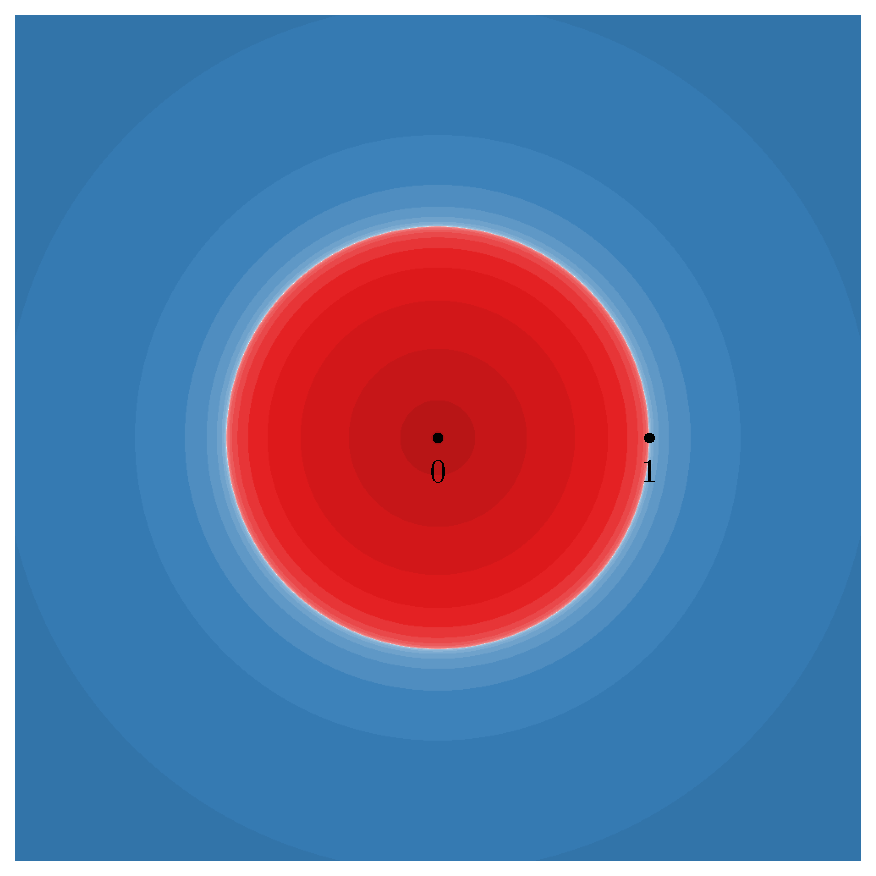
\includegraphics[width=0.5\textwidth]{
        ../figures/z_squared_fatou_basins_and_times.pdf}
    \caption{En rojo se ve el subconjunto de $\ExtC$ que converge a $0$, y en
    azul el que converge a $\infty$. Cuanto más oscuro es el color de un punto 
    más rápido converge su órbita. En blanco se ve la circunferencia unidad.}
    \label{fig:z_squared_fatou_basins_and_times}
\end{figure}

Primero, notemos que $|z^2| = 1$ si y sólo si $|z| = 1$. Esto implica que todo
punto de $C$ tiene todo su futuro en $C$, $R(C) \subseteq C$, y también toda su
historia, $R^{-1}(C) \subseteq C$. Diremos que $C$ es positivamente y
negativamente invariante, o completamente invariante.

\begin{definicion}[Conjunto invariante]
    Dados un conjunto $X$ y una función, $g \colon X \to X$, un
    subconjunto $E$ de $X$ es:
    \begin{enumerate}
        \item positivamente invariante si $g(E) = E$;
        \item negativamente invariante si $g^{-1}(E) = E$;
        \item completamente invariante si $g(E) = E = g^{-1}(E)$.
    \end{enumerate}
\end{definicion}

Aunque sabemos que las órbitas de puntos en la circunferencia unidad nunca salen
de esta, el comportamiento de $R^n(z)$ para cada $z$ en $C$ es complicado. De
hecho, podemos encontrar dos conjuntos densos en $C$ con comportamientos
completamente diferentes. Es decir, dado dos puntos $z_0$ y $w_0$ en $C$, por
muy juntos que estén, podrían describir comportamientos radicalmente distintos.

Las órbitas de los puntos de la forma
\begin{equation}\label{eq:xSquaredType1point}
    \exp(2\pi r i \ 2^m),
\end{equation}
con $r$, $m$ enteros acabarán convergiendo a $1$ en un número finito de pasos.
Cómo todo $z \in C$ se puede expresar en la forma $z = \exp(i\theta)$, tenemos
$R^n(z) = \exp(2^n i\theta)$. Luego, si $z$ es de la forma~
\ref{eq:xSquaredType1point}, para todo $n \geq m$, $R^n(z) = 1$.

Sin embargo, si $z \in C$ no es de la forma~\ref{eq:xSquaredType1point}, se
puede ver que su órbita nunca converge \cite[6]{Beardon1991}. Es más, puede que
$z$ forme una órbita densa en $C$ \cite[8]{Beardon1991}.